\documentclass[12pt, letterpaper]{article}

% Packages
\usepackage[utf8]{inputenc}
\usepackage{tikz}
\usepackage{amsmath}
\usepackage{cprotect}

% Metadata
\title{Context-free grammars and manual procedures for parsing languages}

\author{Jakab Zeller}

\date{October 2021}

% Environments
\newenvironment{tightcenter}{%
  \setlength\topsep{0pt}
  \setlength\parskip{0pt}
  \begin{center}
}{%
  \end{center}
}

\begin{document}

\maketitle

\section{Context-free Grammars}

\subsection{Introduction}

Grammar describes how the strings in a language should be formed according to the language's alphabet and syntax. Grammars contain a set of \textit{production rules}. These inform the parser how to rewrite a string of symbols to give a string that exists within the language.

\subsection{Production Rules}

A production rule describes a substitution for one symbol with one or many symbols. The production rules for context-free grammars take the form:

\begin{center}
    $A \rightarrow \alpha$
\end{center}

Where $A$ is a \textbf{non-terminal} symbol and $\alpha$ is sequence of \textbf{terminal} or \textbf{non-terminal} symbols. Terminal symbols are the tokens or alphabet of the language which the grammar describes. Non-terminals are recursive definitions which use a sequence of terminal or non-terminal symbols. For instance, in the following grammar:

% Grammar for numbers
\begin{figure}[h]
    \begin{center}    
        \begin{verbatim}
        Digit   ::= 0 | 1 | 2 | 3 | 4 | 5 | 6 | 7 | 8 | 9
        Natural ::= 1 | 2 | 3 | 4 | 5 | 6 | 7 | 8 | 9
        Number  ::= Natural | Number Digit
        \end{verbatim}
        \vspace{-1.5em}
    \end{center}
    \caption{A grammar which describes a language of numbers}
\end{figure}

\pagebreak

Both \verb|Digit| and \verb|Natural| are a \textbf{terminal} symbols as they are exactly the tokens matched by the lexical analyser before being passed to the parser. \verb|Number| is a \textbf{non-terminal} as it can be substituted for the two production rules described above.

\subsection{Features of context-free}

A grammar is defined as context free if the non-terminals on the left hand side of each production rule can always be substituted for the right hand side, \textit{regardless of the context of the non-terminal}. Any grammar which does not follow this rule is classified as a \textbf{context-sensitive} grammar.

Most natural languages are defined by a context-sensitive grammar due to things such as the existence of many grammatical cases for the same word that depends on context.

One such example in the English language could be the sub-sentence \textit{"burnt like hell"}. When used in this sentence:

\begin{center}
    "The toast was burnt like hell"
\end{center}

\textit{Burnt} is an \textbf{adjective} applied to the noun. Whereas in:

\begin{center}
    "The fire burnt like hell"
\end{center}

\textit{Burnt} is a \textbf{verb}. The grammar of the word \textit{burnt} would be impossible to describe using a context-free grammar as the \textbf{meaning} of the word depends on the \textbf{context} of the words surrounding it.

\textbf{Deterministic context-free languages}, a subset of context-free languages, can all be recognised by non-deterministic pushdown automaton. This means that all deterministic context-free languages are admitted by unambiguous grammar. Therefore, the parse tree produced by the parser for a deterministic context-free grammar is always unique for every valid input string. Deterministic context-free languages are revered by computer scientists as they can be parsed in linear time by $LR(k)$ parsers, but producing a grammar for them which \textbf{doesn't} actually accept a \textbf{non}-deterministic language instead, is hard to synthesise. This is usually due to:

\begin{enumerate}
    \item Ambiguous grammar being hard to spot with the untrained eye
    \item The dangling-else problem
    \item Not implementing precedence rules
\end{enumerate}

\subsection{Tangent: Where do context-free grammars lie in the grand scheme of formal languages?}

An interesting tangent to dive into is the difference between context-free grammars and other types of grammars. The set of all grammars can be described as a hierarchy known as the \textbf{Chomsky hierarchy} or the \textbf{Chomsky–Schützenberger hierarchy}.

% Chomsky hierarchy
\begin{figure}[h]
    \begin{center}
        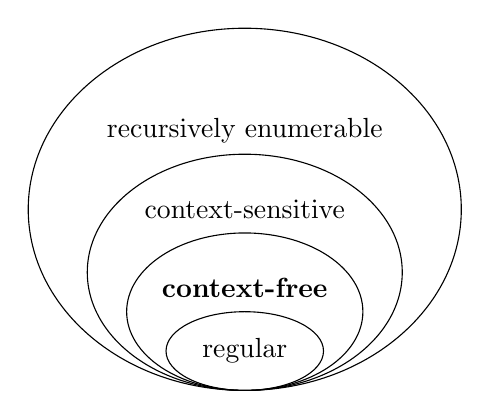
\begin{tikzpicture}
            \node[] at (2,2) {regular};
            \draw (2,2) ellipse (1cm and 0.5cm);
            \node[] at (2,2.8) {\textbf{context-free}};
            \draw (2,2.5) ellipse (1.5cm and 1cm);
            \node[] at (2,3.8) {context-sensitive};
            \draw (2,3) ellipse (2cm and 1.5cm);
            \node[] at (2,4.8) {recursively enumerable};
            \draw (2,3.8) ellipse (2.75cm and 2.3cm);
        \end{tikzpicture}
        \caption{Chomsky/Chomsky–Schützenberger Hierarchy}
    \end{center}
\end{figure}

\begin{enumerate}
    \item \textbf{Regular grammar}
    \begin{enumerate}
        \item Only single non-terminals can be on the left hand side of production rules
        \item The right hand side of production rules must follow either\dots
        \begin{itemize}
            \item A terminal symbol followed by zero or one non-terminal symbol \textbf{(right regular)}
            \item Zero or one non-terminal symbol followed by a terminal symbol \textbf{(left regular)}
        \end{itemize}
        \item An example of a regular grammar is shown in fig. 1 which is \textbf{right regular}
    \end{enumerate}
    \item \textbf{Context-free}: discussed in section 1.3
    \item \textbf{Context-sensitive}
    \begin{enumerate}
        \item Production rules are in the form:
        \begin{center}
            $\alpha A \beta \rightarrow \alpha \gamma \beta$
        \end{center}
        \item $S \rightarrow \epsilon$ can only exist if $S$ doesn't occur on the right hand side of any production rule
        \item Where $A$ is a non-terminal and $\alpha$, $\beta$, and $\gamma$ are non-terminals or terminals, $\alpha$ and $\beta$ may be empty, and $\gamma$ must be non-empty.
        \item The English language is an example of a context-sensitive language
    \end{enumerate}
    \item \textbf{Recursively enumerable}: are all languages that can be recognisable by Turing machines and encompass all formal languages
\end{enumerate}

\pagebreak

\section{Manual Parsing Techniques}

When it comes to parsing algorithms they are split into two main groups: \textbf{top-down} parsers and \textbf{bottom-up} parsers. This relates to the way that the \textbf{parse tree} is constructed for a given input string.

A \textbf{parse tree} is a rooted tree which represents the syntactic structure of an input string. The grammar accepted by parsers which generate a parse tree must have a non-terminal root symbol which encompasses the entire input string as well as terminal symbols which form the leaf nodes of the tree. In other words, a context-free grammar.

Practically, parse trees can be used passed into a semantic analyser to produce an Abstract Symbol Tree (AST), which can then be traversed to produce code in a compiled language or executed directly in an interpreted language.

\subsection{A note on derivations}

Given an input string $S$ and a grammar $G$, the derivation of $S$ on grammar $G$ is one of the possible sequences of grammar rules that must be applied to transform the start symbol into $S$. Thus, proving that the string $S$ belongs in the language defined by grammar $G$.

For instance, given the following grammar describes the syntax that could be accepted by a four function calculator:

% Grammar for four function calc
\begin{figure}[h]
    \begin{center}
        \begin{verbatim}
            E ::= T | E A
            A ::= "+" T | "-" T
            T ::= F | T P
            P ::= "*" F | "/" F
            F ::= N | (E)
            N ::= Z | N D
            Z ::= 1 | 2 | 3 | 4 | 5 | 6 | 7 | 8 | 9
            D ::= 0 | 1 | 2 | 3 | 4 | 5 | 6 | 7 | 8 | 9
        \end{verbatim}
    \end{center}
    \vspace{-1.5em}
    \caption{Grammar describing the syntax of a four function calculator}
\end{figure}

\pagebreak

One of the possible derivations for the string \verb|1 + 2 * 3| with the start state $E$ could be...

% Possible derivation of "1 + 2 * 3" with start symbol E
\begin{figure}[h]
    \begin{equation}
        \begin{split}
            E &\rightarrow EA\\
            &\rightarrow TA\\
            &\rightarrow FA\\
            &\rightarrow NA\\
            &\rightarrow ZA\\
            &\rightarrow 1 A\\
            &\rightarrow 1 + T\\
            &\rightarrow 1 + TP\\
            &\rightarrow 1 + FP\\
            &\rightarrow 1 + NP\\
            &\rightarrow 1 + ZP\\
            &\rightarrow 1 + 2 P\\
            &\rightarrow 1 + 2 * F\\
            &\rightarrow 1 + 2 * N\\
            &\rightarrow 1 + 2 * Z\\
            &\rightarrow 1 + 2 * 3
        \end{split}
        \nonumber
    \end{equation}
    \vspace{-1.5em}
    \cprotect\caption{A possible derivation of \verb|1 + 2 * 3| with start state $S$ on the grammar given in fig. 3}
\end{figure}

This derivation is a \textit{leftmost derivation}, which means that it always derives the leftmost non-terminal. It is also a derivation of an \textbf{ambiguous} grammar which means that this derivation belongs to the set of all possible derivations. Each possible derivation can be treated as different subtree whenever a production rule with no terminals on the right hand side is used.

\subsection{Top-down vs. Bottom-up parsing}

\subsubsection{Top-down}

\subsubsection{Bottom-up}

% Describe the shift-reduce algorithm and give an example

% Bibliography

% https://www.inf.ed.ac.uk/teaching/courses/inf2a/slides2016/inf2a_L29_slides.pdf
% https://homepages.dcc.ufmg.br/~hbarbosa/teaching/uiowa/toc/notes/10-dcfl.pdf

\end{document}
